%%% -*-LaTeX-*-

\chapter{Solution Counting}

Currently, SweetPea offloads the entire sampling process to an external tool. While an attractive option from an implementation standpoint, this approach does not scale to the sizes needed. As demonstrated in chpater two, the problem spaces that SweetPea is trying to sample from are beyond the capacity of any existing tools. One of the shortcomings of this approach is that external tools cannot take advantage of knowledge of the problem to guide their decisions.

Experimental designs in SweetPea can be viewed as combinatorics problems, each with a countable set of solutions. If we could construct a formula for counting the solutions to an experimental design, we may be able to also discover a bijection between solutions to the design and the natural numbers. This would reduce the burden of guaranteeing uniformity to randomly sampling natural numbers from the uniform distribution.

As a first foray into solution counting for SweetPea designs, this section only considers tier 1, 2, and 3 designs. We also leave the set of design constraints for later consideration.


\section{Principles of Counting}

Before describing a formula for counting solutions to experimental designs, it will be useful to review a few counting principles for future reference, beginning with counting permutations of a set. The standard formula for then number of permutations of $r$ items taken from an $n$-element set is:

\[
P(n,r) = \frac{n!}{(n-r)!}
\]

See \cite{brualdi_introductory_2010}. When $n =  r$, this becomes simply $n!$.

% Similary, the number of combinations of $r$ items from an $n$-element set is:

% \[
% {n \choose r} = \frac{n!}{r!(n-r)!}
% \]

When constructing a set $S$ by combining individual elements from mulitple other sets, $P_1, P_2, \cdot\cdot\cdot P_n$, the size of $S$ is the product of the sizes of sets $P_1, P_2, \cdot\cdot\cdot P_n$:

\[
|S| = \prod_{i=1}^n |P_i|
\]

This is known as the \textit{Multiplication Principle} \cite{brualdi_introductory_2010}.


\section{Partition of an Experimental Design}

An experimental design is composed of three elements: a set of factors, a subset of the factors to be combined with each other (crossed), and a set of constraints. The set of crossed factors fundamentally shape the generated trial sequences. The length of a trial sequence is governed by the number of combinations of level values for each crossed factor. For example, consider a design in which there are two crossed factors, each with three levels. By the multiplication principle, there are $3 * 3 = 9$ unique combinations of level values from each factor, hence trial sequences in this design will be nine trials long.

Let $D$ be the set of all factors in the design. Let $C$ be the set of crossed factors, and $\overline{C}$ be the set of factors not included in the crossing. Therefore $C \subseteq D$ and $\overline{C} \subset D$. $C$ and $\overline{C}$ can both be further divided based on the type of factor: basic or derived. Let $C_B$ be the set of basic factors in $C$, and $C_D$ be the set of derived factors in $C$. We will define $\overline{C}_B$ and $\overline{C}_D$ similarly for $\overline{C}$.

Lastly, we further divide $\overline{C}_B$ into two more sets. Although basic factors in $\overline{C}$ are not included in the set of crossed factors, this does not imply that they are fully independent. It is possible that factors in $C_D$ depend on factors in $\overline{C}_B$. We'll refer these factors in $\overline{C}_B$ as \textit{source} factors, as they are at least a partial source of the data controlling factors in $C_D$. We will group such factors in $\overline{C}_{B_S}$, while $\overline{C}_{B_I}$ represents the truly independent basic factors in $\overline{C}$.

We could also define $C_{B_S}$ and $C_{B_I}$, however there will be no benefit to doing so, as the relationship between factors in $C_B$ and dependent derived factors is inverted. Each combination of levels in the crossed set governs the values for $C_B$, which will then in turn govern dependent derived factors.

The partition of $D$ with which we are concerned is therefore: $\{C_B, C_D, \overline{C}_{B_S}, \overline{C}_{B_I}, \overline{C}_D\}$, as shown in figure \ref{fig:partition}.

% \begin{figure}[t]
% \centering
% \centerline{\includegraphics[origin=c,width=12cm]{../figures/partition.jpg}}
% \caption{Partition of an Experimental Design}
% \label{fig:partition}
% \end{figure}

\begin{figure}[t]
\centering
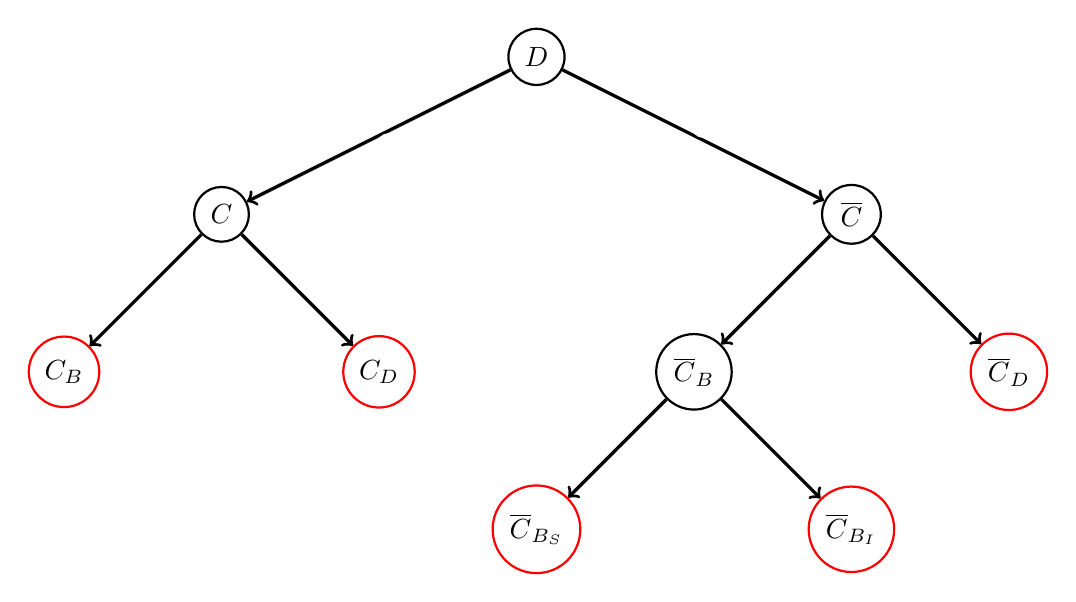
\begin{tikzpicture}[auto]
\begin{scope}[every node/.style={circle,thick,draw}]
    \node (D) at (8,8) {$D$};

    \node (C) at (4,6) {$C$};
    \node (CBar) at (12,6) {$\overline{C}$};

    \node[draw=red] (CB) at (2,4) {$C_B$};
    \node[draw=red] (CD) at (6,4) {$C_D$};
    \node (CBarB) at (10,4) {$\overline{C}_B$};
    \node[draw=red] (CBarD) at (14,4) {$\overline{C}_D$};

    \node[draw=red] (CBarBS) at (8,2) {$\overline{C}_{B_S}$};
    \node[draw=red] (CBarBI) at (12,2) {$\overline{C}_{B_I}$};
\end{scope}

\begin{scope}[every node/.style={fill=white,circle},
              every edge/.style={draw=black,very thick}]
    \path [->] (D) edge node {} (C);
    \path [->] (D) edge node {} (CBar);

    \path [->] (C) edge node {} (CB);
    \path [->] (C) edge node {} (CD);

    \path [->] (CBar) edge node {} (CBarB);
    \path [->] (CBar) edge node {} (CBarD);

    \path [->] (CBarB) edge node {} (CBarBS);
    \path [->] (CBarB) edge node {} (CBarBI);
\end{scope}
\end{tikzpicture}
\caption{Partition of an Experimental Design}
\label{fig:partition}
\end{figure}

Lastly, we define $X$ to be a set of ordered pairs $t_1, t_2, \cdot\cdot\cdot t_n$, representing the crossing of factors in $C$. Each ordered pair $t$ contains items $i_1, i_2, \cdot\cdot\cdot i_j$, where item $i_j$ is one of the levels from the $j_{th}$ factor in $C$. Each ordered pair $t$ must be unique, and there is an ordered pair for every possible combination of levels from factors in $C$. By the multiplication principle, there will be $n = C_1 \cdot C_2 c\dot\cdot\cdot C_{|C|}$ such ordered pairs, and there are $P(n, n) = n!$ permutations of this set. We will also use $l$ to refer to the trial sequence length, which is equivalent to $|X|$.


\section{Formula}

With the partition established, we are now able to develop the formula for counting the number of solutions, $s$, for an experimental design. For the simplest of designs (tier 1), the ordered pairs in $X$ fully represent all possible trials. $C_B \neq \emptyset$, while every other set in the partition is empty. Every permutaion of $X$ represents a unique trial sequence, therefore there are $s = l!$ solutions to a tier 1 design.

Tier 2 designs introduce basic factors that are not in $C$, and are thus less constrained. In otherwords, starting with tier 2, $\overline{C}_{B_I} \neq \emptyset$. For a factor $f$, let $|f|$ denote the number of levels that $f$ has. For each $f \in \overline{C}_{B_I}$, $f$ is fully independent; therefore, any of the $|f|$ levels may be selected for each trial. In a sequence of $l$ trials, we can again apply the multiplication principle to determine that there are $|f|^l$ possible combinations of the levels of $f$. If $|\overline{C}_{B_I}| > 1$, then we apply the multiplication principle repeatedly to determine the total number of combinations for all factors in $\overline{C}_{B_I}$. Applying the multiplication principle one more time, we see that the total number of solutions for a tier 2 design is:

\[
s = l! \cdot \prod_{i=1}^{|\overline{C}_{B_I}|} |f_i|^l
\]

% TODO: Comment on the fact that a user can specify an unsatisfiable crossing, in which the solution count is 0.
% The solver detects this in practice.

% TODO: End of 4.3: It's not immediately obvious that computing the level-3
% solution-space size is tractable, but I think SweetPea's implementation
% relies on being able to do this (i.e., I think it builds up a truth
% table by trying every combination in the crossing). Some words of
% clarification or explanation would be helpful.

With tier 3 designs come derived factors. It is now possible that all sets in the partition are non-empty. The only sets in the partition that we have yet to consider are $C_D$, $\overline{C}_{B_S}$, and $\overline{C}_D$. The presence of factors in $C_D$ does not alter the formula, as level selection for factors in $C_D$ is still controlled by $X$ (the crossing). $\overline{C}_D$ also requires no special treatment as the level selection for its factors depends entirely on the levels selected for basic factors. (Whether in $C_B$, $\overline{C}_{B_S}$, or $\overline{C}_{B_I}$.) This leaves only $\overline{C}_{B_S}$, which will be our next focus.

Derived factors allow the user to provide an arbitrary predicate for each level in the factor. We have not solved the halting problem, so we will need to apply these predicates to different argument combinations in order to determine which inputs are acceptable for each trial. We define $X_S$ to be the set of ordered pairs representing the crossing of factors in $\overline{C}_{B_S}$, also referred to as the \textit{source crossing}. The next task is to determine, for every element in $X$, which elements of $X_S$ are compatible using the user-defined predicates.

For every ordered pair $t \in X$, there is some number of items in $t$ corresponding to derived factor levels, labeled $d_1, d_2, \cdot\cdot\cdot d_{|C_D|}$ comprising the set $V_t$. Each $d \in V$ is associated with a predicate\footnote{These predicates, also called derivation functions, are expected to be deterministic. If they are non-deterministic, then inconsistent solutions may be produced as the predicates may be applied more than once to the same arguments. This could also be handled by ensuring that each predicate is only applied once to each argument combination and the results are saved.}, $pred(d)$. For every $t \in X$, every $b \in X_S$ is consulted to see if the predicates for all $d \in V_t$ are satisfied. If any one of them is not satisfied, then $b$ is not a compatible choice for $t$, and must be discarded from consideration for $t$. Once this process is complete, we are left with a list of subsets of $X_S$, in which the $n^{th}$ subset indicates which elements of $X_S$ are compatible with the $n^{th}$ crossing in $X$.

More formally, let $S$ be a list of items $J_1, J_2, \cdot\cdot\cdot J_{|X|}$. The following statements are true:

\begin{enumerate}
\item $\forall J \in S \mid J \subseteq X_S$
\item $\forall t \in X,  \forall d \in V_t \mid pred(d) \implies \top$
\end{enumerate}

Once we have generated $S$, we can apply the multiplication principle one more time to complete the formula for tier 1, 2, and 3 designs:

\[
s = l! \cdot \prod_{i=1}^{|\overline{C}_{B_I}|} |f_i|^l \cdot \prod_{k=1}^{|S|} |J_k|
\]

The total number of solutions $s$ for an experimental design, is the product of the number of permutations of the crossed factors, the number of combinations of each independent factor, and the number of acceptable combinations of all source factors.


\section{Example}

TODO

% TODO: Correctness proof? MEntion that counts have been tested with SAT model counters?
